
\section{Decision Tree}\label{sec:decision-tree}

An implementation introduced in~\cite{bot_or_human} uses the C4.5 decision tree algorithm to determine if a user is a bot or not by characterizing human behaviors from bot behaviors in online services.
This approach consists of a two-step system that (1) extracts a user's behavioral metrics via a client-side logger, and (2) determines the botness of a user, based on the retrieved behavioral metrics, with a server-side classifier.
A client-side logger, in this context, records a user's behavioral metrics such as mouse movements and keystrokes.
Upon gathering this client-side data, the records are sent to the server-side classifier that utilizes the C4.5 decision tree algorithm.

There are two different bot detection approaches that this article seeks to address.
Firstly, \textbf{content-based filtering}, used by third party clients, needs to be improved upon since they suffer from high false negative rates.
This is due to mostly in part of the bot makers finding ways to evade filtering rules set by enforcers.
Secondly, \textbf{human interactive proofs} (HIP)s, such as CAPTCHA, are problematic for more than one reason.
Not only are CAPTCHAs breakable by bot implementors, but the they are intrusive to the user experience.
Although there are ways to increase the reliability of HIPs to detect and block bots, such ways would require more interaction from the authentic human users, thus increasing user friction and diminishing the user experience.
Human observational proofs (HOB)s are a solution to this dilemma.
Unlike the HIPs that are commonly used, HOPs passively observe the actions and behavior of users performing tasks that are meant to be challenging for bots.

A blog site was the testing location for this research.
With over 65,000 users, averaging about 800 users simultaneously online, human user sessions were recorded to describe the various behavior characterizations.
Additionally, bot profiles were generated under 3 distinct categories (ranked by level of sophistication):
\begin{enumerate}
    \item \textbf{replay}: the most sophisticated type of bot, thus making it the most difficult bot to detect among the other 2 types.
        This bot records the actions of a human user doing something on the website, such as filling out a form or clicking on a button.
        Then the bot will impersonate that human user by replaying the recorded actions, exactly following the keystroke and mouse movement styles of that user.
    \item \textbf{mimic}: since most standard bot detection schemes use keystroke and mouse movement info, or the lackthereof, of the user to determine their botness, bot implementors need to include such details in their mimicking bot schemes.
        Using OS API calls to generate keystroke and mouse events, mimicking bots are able to bypass older or standard detection schemes.
        This is possible when a detection scheme only relies on UI events, such as mousemove, keystrokes, etc., which can be triggered by either hardware, such as a mouse and keyboard, or software, such as the OS API calls a mimicking bot would utilize.
    \item \textbf{inject}: while being the most common type of bot, this type of bot does not interact with the UI. Instead, it triggers the same code that UI events would tirgger, such as an HTTP request that would regularly be triggered by clicking on a UI button.
        Despite being detectable by most bot detection schemes, injection bots are still able to evade a server's check on HTTP protocols by forging certain fields in the headers, such as Referer, User Agent, and Cookie.
\end{enumerate}
While human user behavioral characterization data was collected from 1,078 signed-in site members during several two-hour monitoring sessions, bot user behavioral characterization data was collected by using existing libraries and frameworks.
For the injection bots, any UI features that triggered a POST request were instead triggered by cURL and a predifined string for the request body.
An open source Windows program, AutoHotkey, that is designed for automating the Windows GUI and for general scripting was used to configure the mimicking bot.
The AutoHotkey script they used was customized to the blog site, mimicking all sorts of human actions, such as moving, clicking, and scrolling the mouse cursor, as well as typing keys.
All mimicked actions were masked by entropies, such as random speeds of mouse movements or random delays when typing, to create some sort of human-like characteristics.
With the ability to record and replay mouse and keyboard API calls, the Global Mouse and Keyboard Library for Windows was used to configure the replay bot.

Their detection system design consists of a webpage-embeded logger, that records a user's behavior on the client-side, and a server-side classifier that considers the user's data from the client-side and determines if that user is a bot or not.
\begin{figure}[!h]
    \centering
    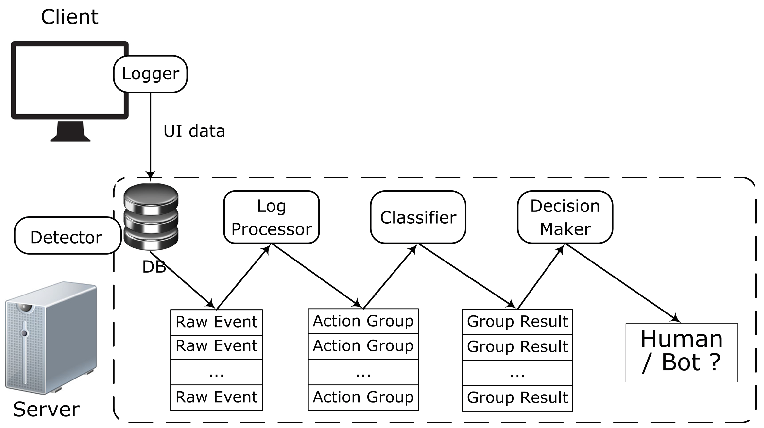
\includegraphics[width=.8\columnwidth]{figures/bot_or_human_system_architecture}
    \caption{Architecture of the client-side Logger and server-side Detector}
    {\small The client-side Logger and server-side Detector setup above, as shown in~\cite{bot_or_human}, closely resemble that of this thesis work's system design.}
    \label{fig:bot-or-human-architecture}
\end{figure}
Similarly to this thesis research implementation, the client-side Logger is JavaScript code that stores UI event recordings into a buffer and periodically POSTs data to the server.
Mouse metrics are recorded at an average of 125hz polling rate.
Unbeknownst to the user, the Logger collects, via JavaScript events, five UI events: \textit{key press}, \textit{key release}, \textit{mouse move}, \textit{mouse button press}, and \textit{mouse button release}.
When the recordings are POSTed to the server-side Detector, a \textbf{log processor} begins to calculate the timing entropy of intervals of the whole raw event data sequence in the POSTed user log.
This detects periodic or regular timing of the entire user behavior.
The entropy rate can be used to distinguish a human user from a bot user.
Human behavior is often more complicated than bot behavior.
Such complexity can be measured by the entropy rate.
Once the log processor finishes, the C4.5 algorithm is used as a base for the Detector's \textbf{classifier}.
Reasons for using the C4.5 decision tree algorithm include its efficiency to process large amounts of training data in a short time, the logic is easy to understand and not a black-box, the tree is able to process continuous and discrete values, and lastly, the tree has autonomous tree height constraints to avoid over fitting.
Finally, the \textbf{decision maker} in the Detector considers all classifications previously made on a user, and holistically makes a decision of its botness.
